\documentclass[pdf, hyperref={unicode}, aspectratio=169]{beamer}

\usepackage{./diploma-slides-latex-template/styles}

% Включаю кнопочки
\setbeamertemplate{navigation symbols}[default]

% Название темы слишком длинное, поменьше шрифт!
\setbeamerfont{title}{series=\bfseries, size=\large}
\setbeamerfont{footline}{series=\bfseries, size=\fontsize{5}{3}\selectfont}

\useoutertheme{miniframes}

\title{Проектирование системы переноса и генерации взаимосвязанных данных из производственной среды при тестировании образовательной платформы}

\subtitle{Выпускная квалификационная работа бакалавра}

\pdfstringdefDisableCommands{
\def\\{}
\def\,{}
\def\textbf#1{<#1>}
}

\author[Мезенин Олег Александрович]
{
	\textbf{Студент группы М8О-406Б-21:} Мезенин Олег Александрович\\
	\ \textbf{Научный руководитель:} ст. преподаватель кафедры 806\\\ Миронов Евгений Сергеевич
	% Обратите внимание на пробел в начале строки
}

\institute[Московский авиационный институт]
{
	Московский авиационный институт (национальный исследовательский университет)\\
	Институт № 8 «Компьютерные науки и прикладная математика»\\
	Кафедра № 806 «Вычислительная математика и программирование» 
}

\date{Москва --- \the\year}

\logo{
\includegraphics[height=1cm]{img/mai}}


\begin{document}

\epstopdfsetup{outdir=./}

{
	% убирает номер слайда с титульного слайда
	\setbeamertemplate{page number in head/foot}{}
	\frame{\titlepage}
}

\begin{frame}
	\frametitle{Актуальность темы}
	\begin{itemize}
		\item Тестирование программного продукта важно.

		\item Тестирование нельзя проводить в производственной среде:
		\begin{itemize}
			\item лишняя нагрузка на систему;
			\item юридические риски.
		\end{itemize}

		\item Копирование всех данных:
		\begin{itemize}
			\item занимает много времени;
			\item использует много ресурсов.
		\end{itemize}

		\item Для многих тестовых сценариев не нужно много данных, но нужны согласованные данные.
	\end{itemize}
\end{frame}


\begin{frame}
	\frametitle{Цель и задачи работы}
	
	\textbf{Цель} --- проектирование системы, способной переносить взаимосвязанные данные, анонимизировать их и генерировать тестовые данные.

	\textbf{Задачи:}
	\begin{enumerate}
		\item определение требований;
		\item анализ аналогов;
		\item проектирование архитектуры;
		\item разработка алгоритмов переноса и генерации;
		\item разработка языка для описания данных;
		\item реализация минимально жизнеспособный продукт;
		\item анализ результатов.
	\end{enumerate}
\end{frame}


\begin{frame}
\frametitle{Архитектура системы}
	Система переноса и генерации данных

	\begin{center}
		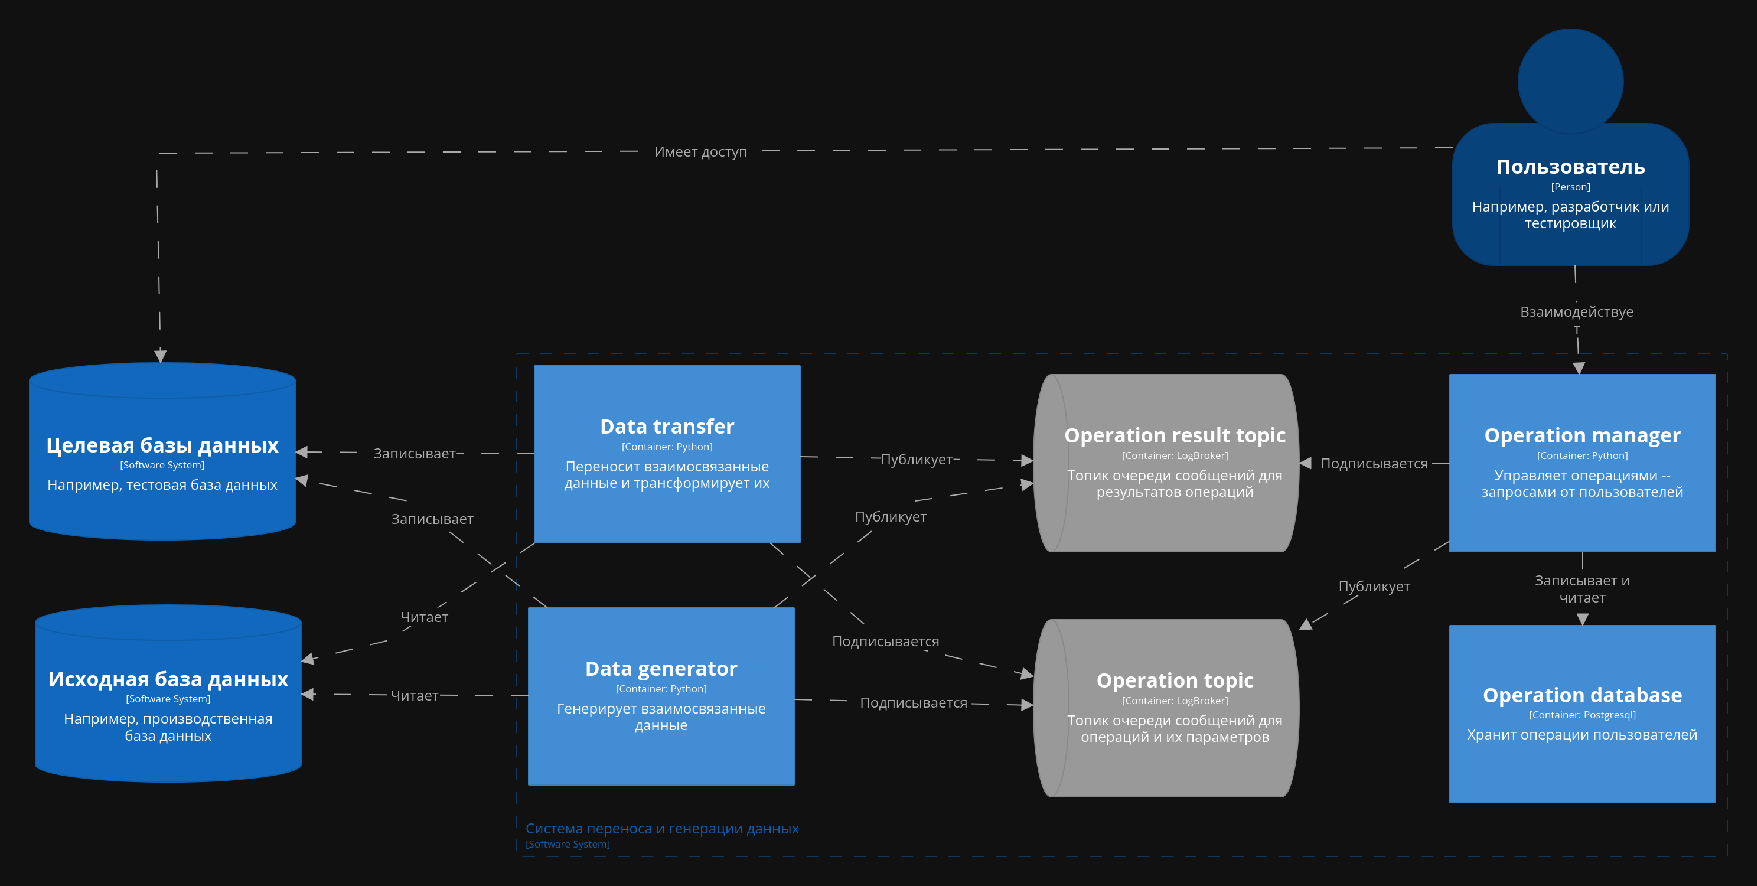
\includegraphics[height = 6cm]{img/structurizr-Containers-cut}
	\end{center}
\end{frame}


\begin{frame}
\frametitle{Архитектура системы}
	Компоненты Data Transfer

	\begin{center}
		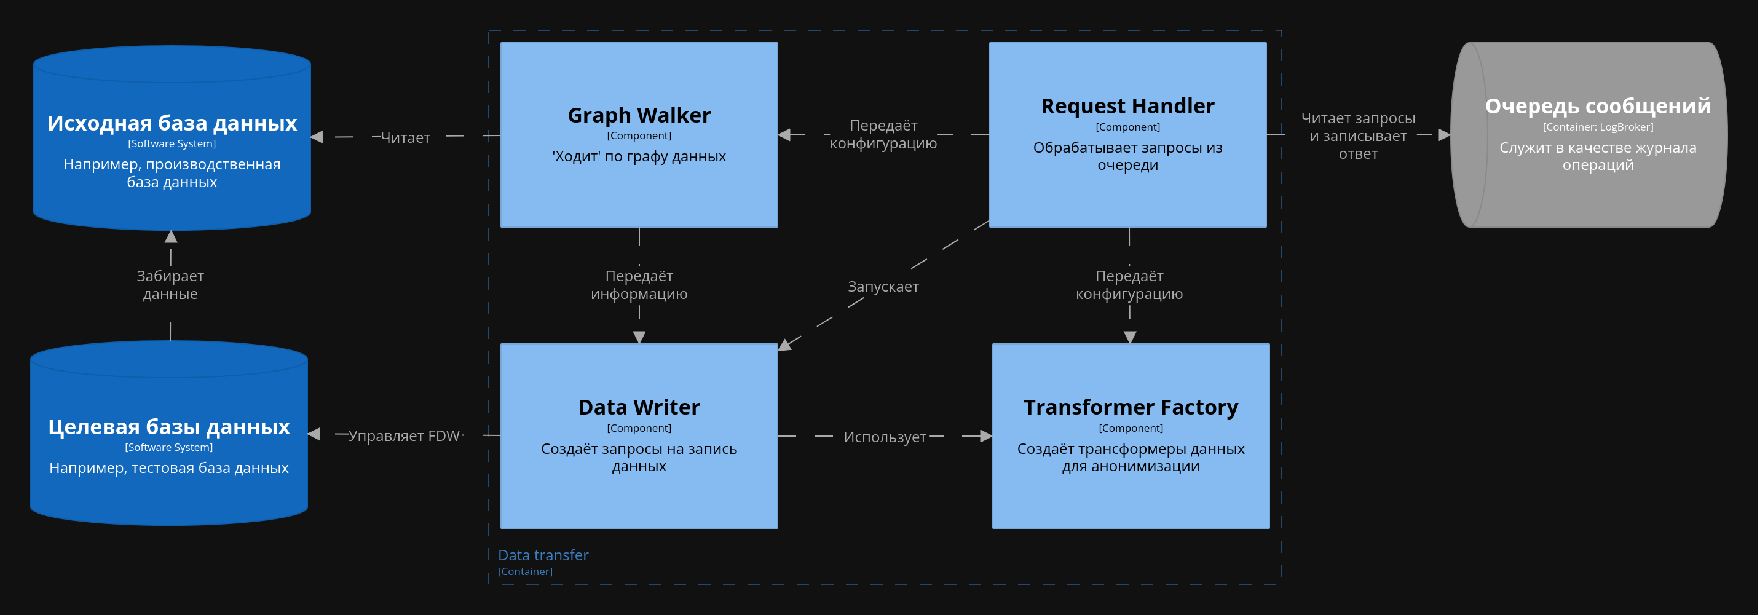
\includegraphics[width = 13cm]{img/structurizr-DataTransferComponents-cut}
	\end{center}
\end{frame}


\begin{frame}
\frametitle{Метаграфы}
	\textbf{Предпосылки} к использованию метаграфов:

	\begin{itemize}
		\item система данных в БД и их взаимосвязей напоминает графовую структуру;
		\item классические графы и ER-модель не подходят ввиду ограниченных возможностей.
	\end{itemize}

	Пусть $MG = \langle V, MV, E, ME \rangle$ -- метаграф, где $V$ -- множество вершин, $MV$ -- множество метавершин, $E$ -- множество рёбер, $ME$ -- множество метарёбер.

	\textbf{Соответствие объектов} в метаграфе и БД:
	\begin{itemize}
		\item вершина $\Leftrightarrow$ запись;
		\item метавершина $\Leftrightarrow$ таблица;
		\item ребро $\Leftrightarrow$ связь между записями;
		\item метаребро $\Leftrightarrow$ логический внешний ключ.
	\end{itemize}
\end{frame}


\begin{frame}
\frametitle{Метаграфы}
	Пример базы данных

	\begin{center}
		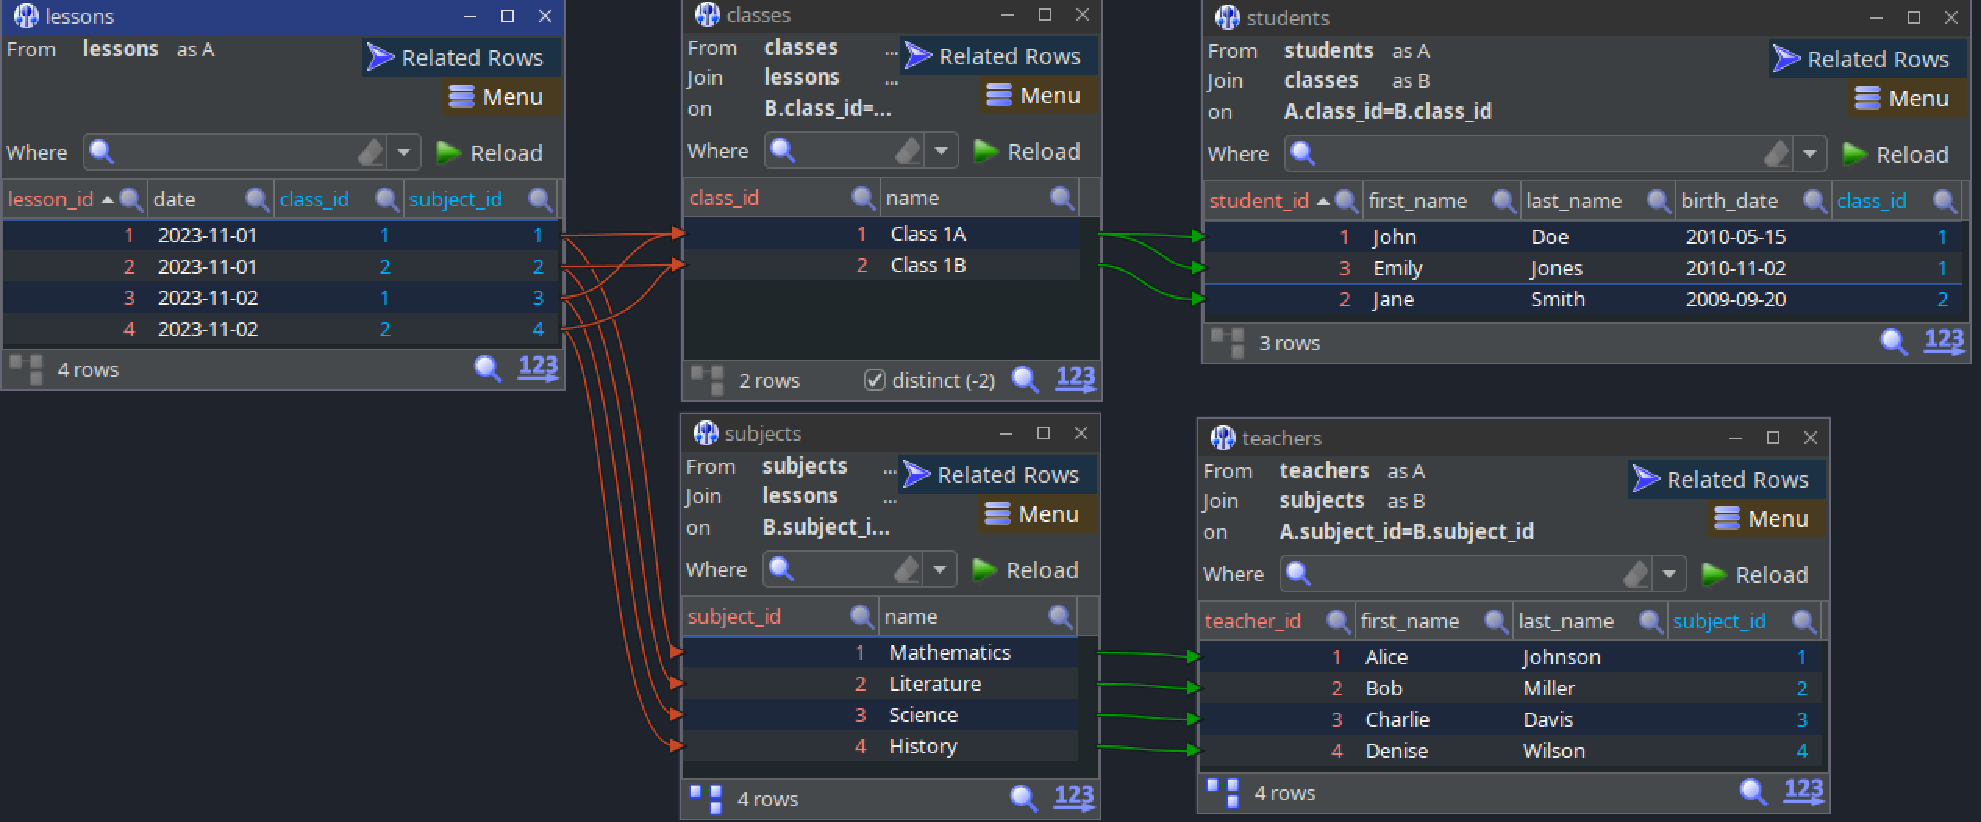
\includegraphics[width = 13cm]{img/jailer-example-db}
	\end{center}
\end{frame}


\begin{frame}
\frametitle{Метаграфы}
	Графическое отображение метаграфа

	\begin{center}
		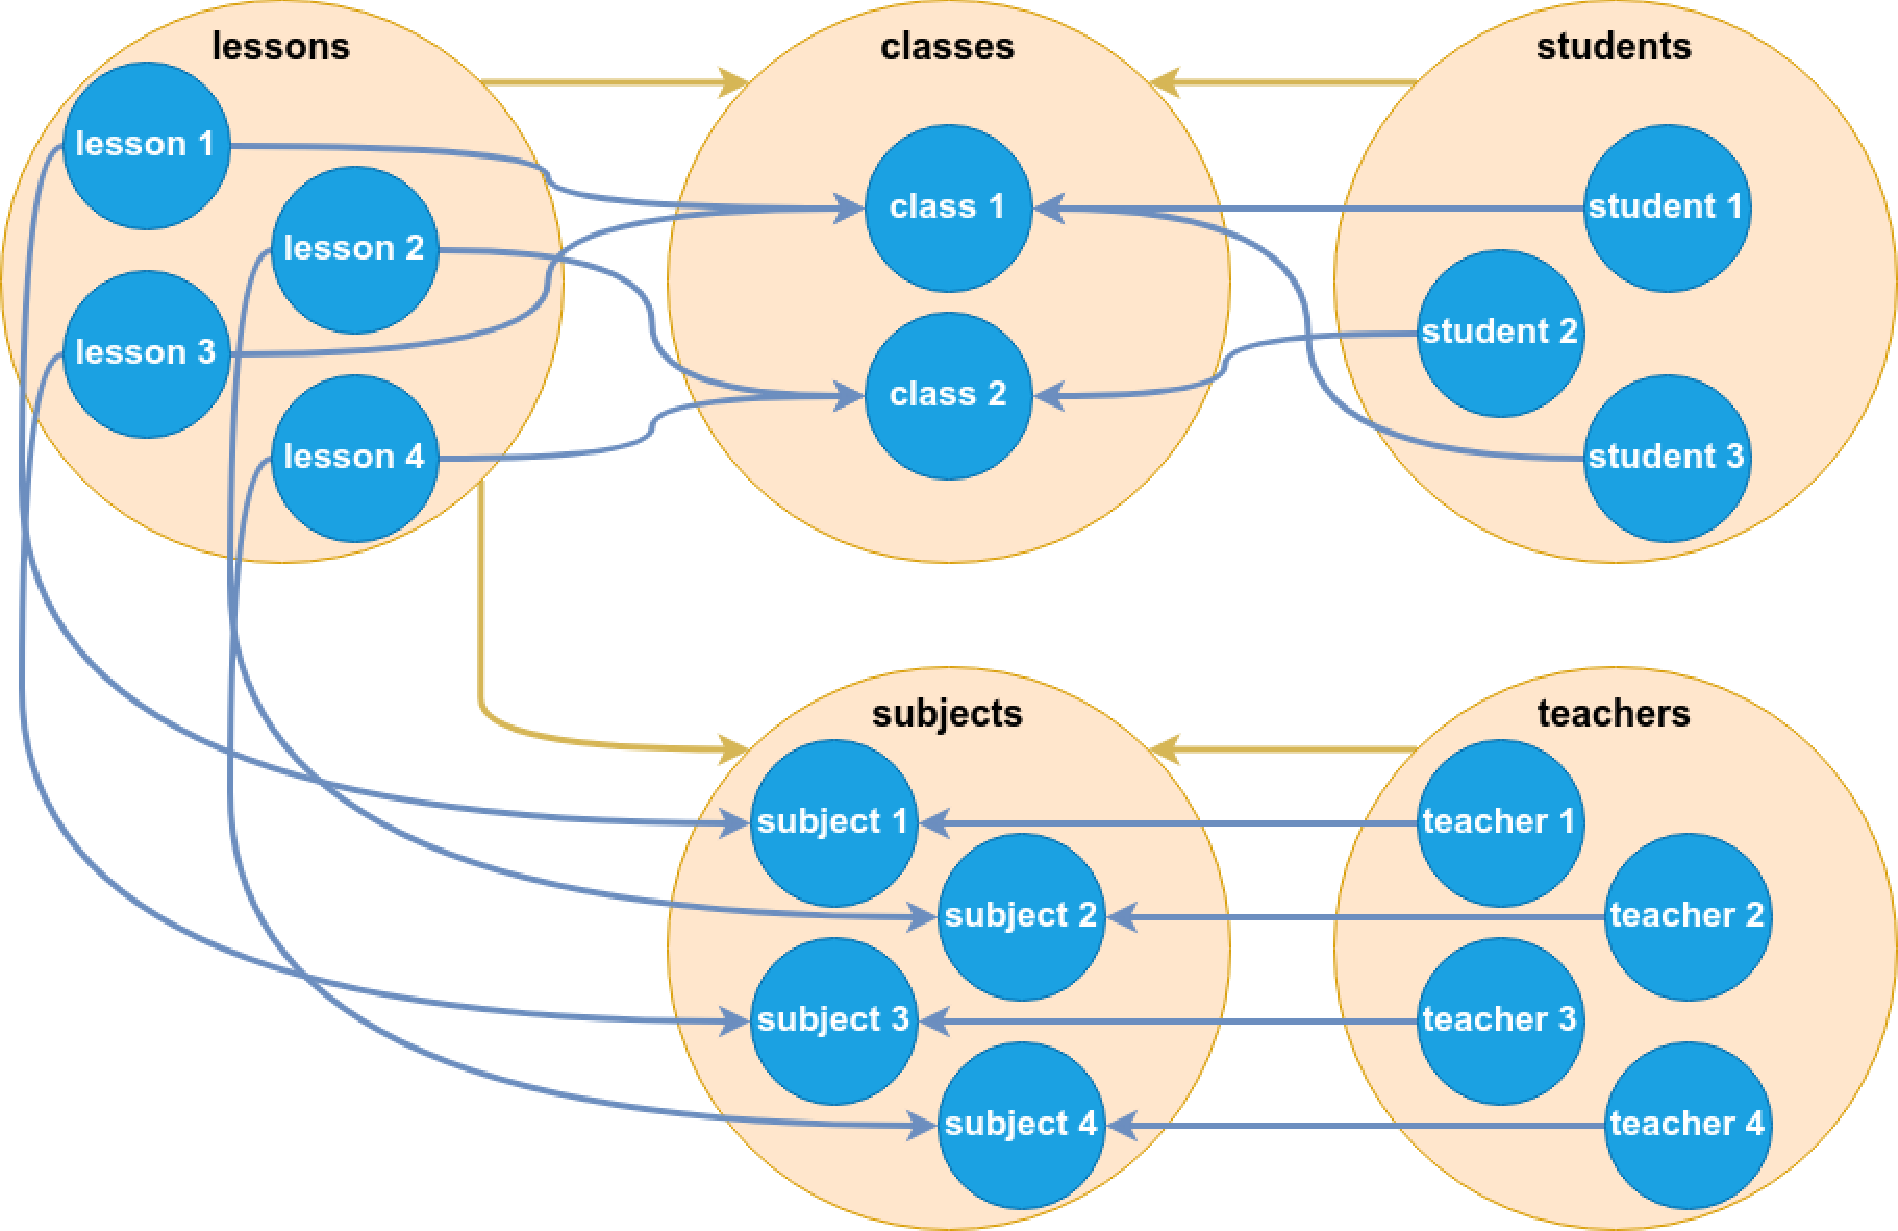
\includegraphics[height = 6cm]{img/drawio-metagraph}
	\end{center}
\end{frame}


\begin{frame}
\frametitle{Правила метаграфа}
	Пусть $r = \langle p, f \rangle$ -- правило метаграфа, где $p$ — предикат, а $f$ — функция, изменяющая множества метаграфа
\end{frame}


\begin{frame}
\frametitle{Алгоритм обхода данных}

	\begin{center}
		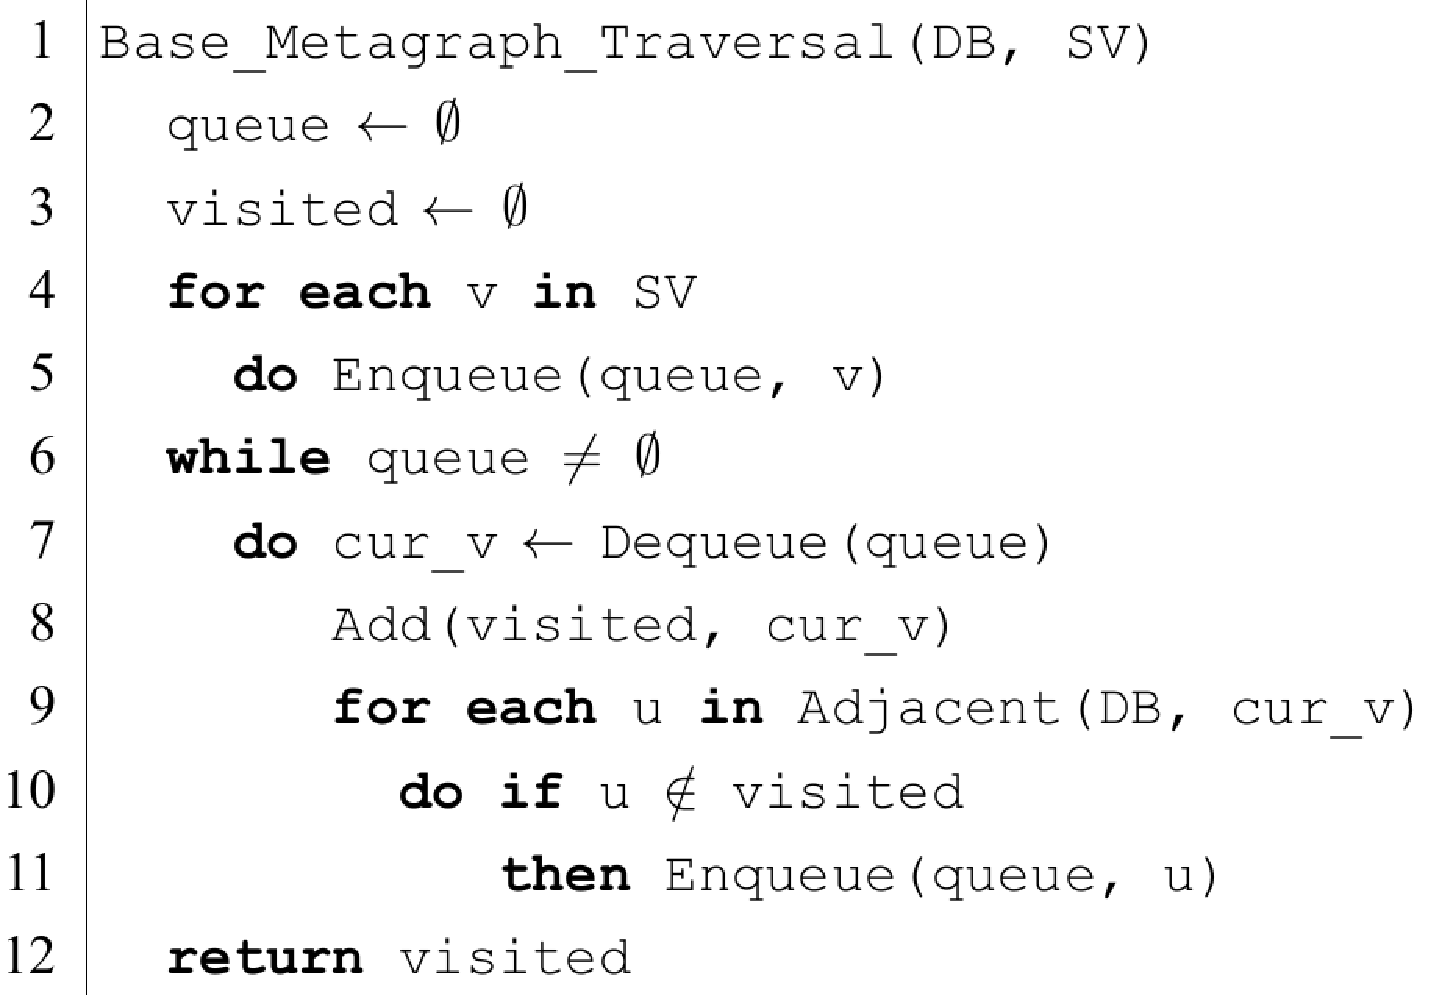
\includegraphics[height = 6.5cm]{img/algorithm-base}
	\end{center}
\end{frame}


\begin{frame}
\frametitle{Алгоритм обхода данных}

	\begin{center}
		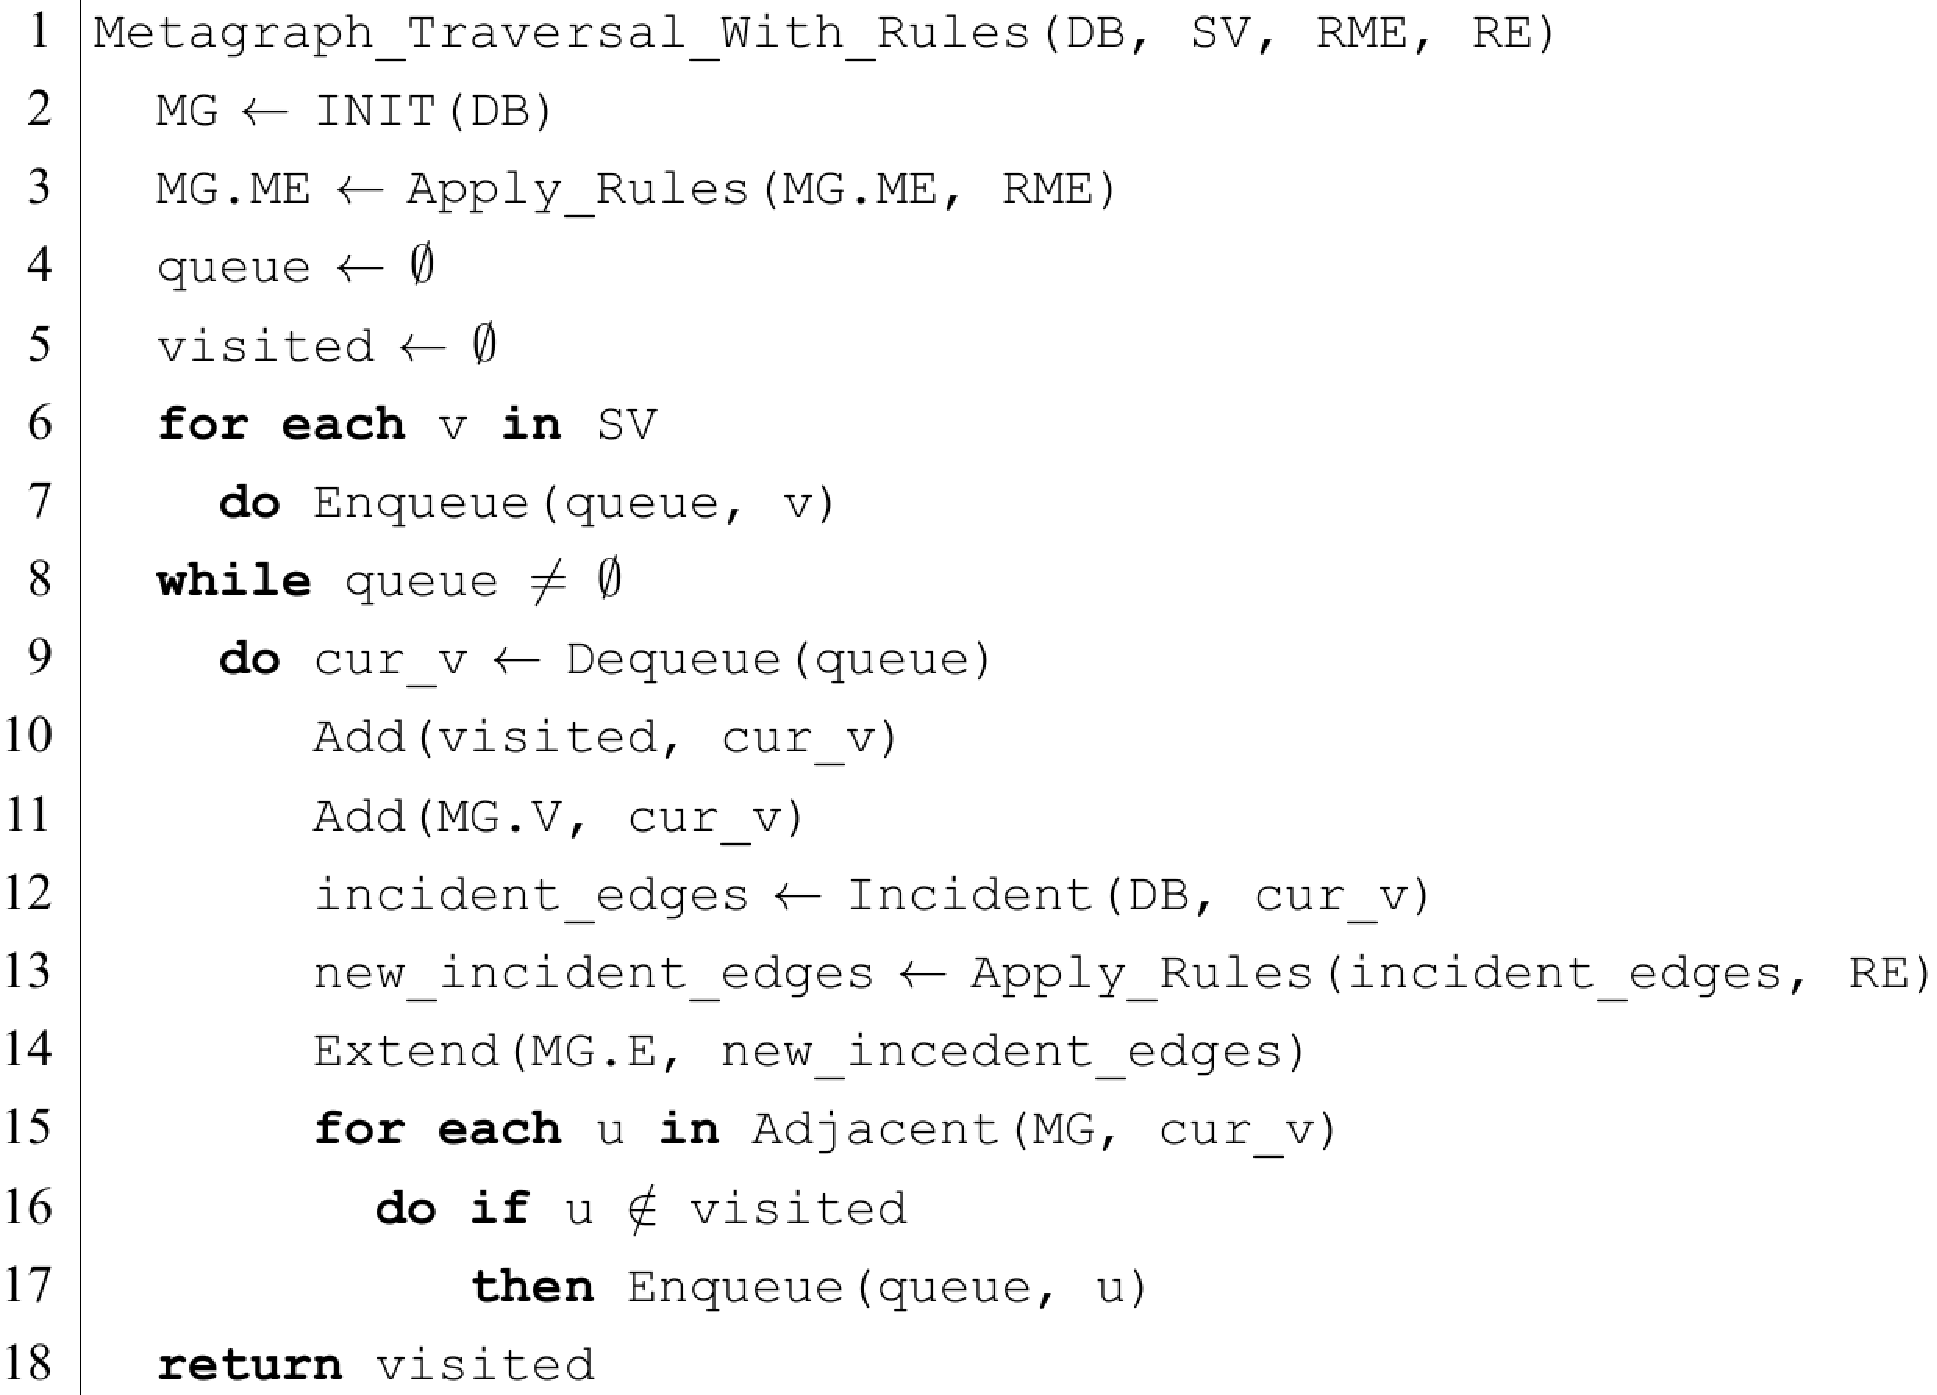
\includegraphics[height = 6.5cm]{img/algorithm-with-rules}
	\end{center}
\end{frame}


\begin{frame}
\frametitle{Язык описания метаданных}
	Примеры грамматических конструкций на ANTLR4

	\begin{center}
		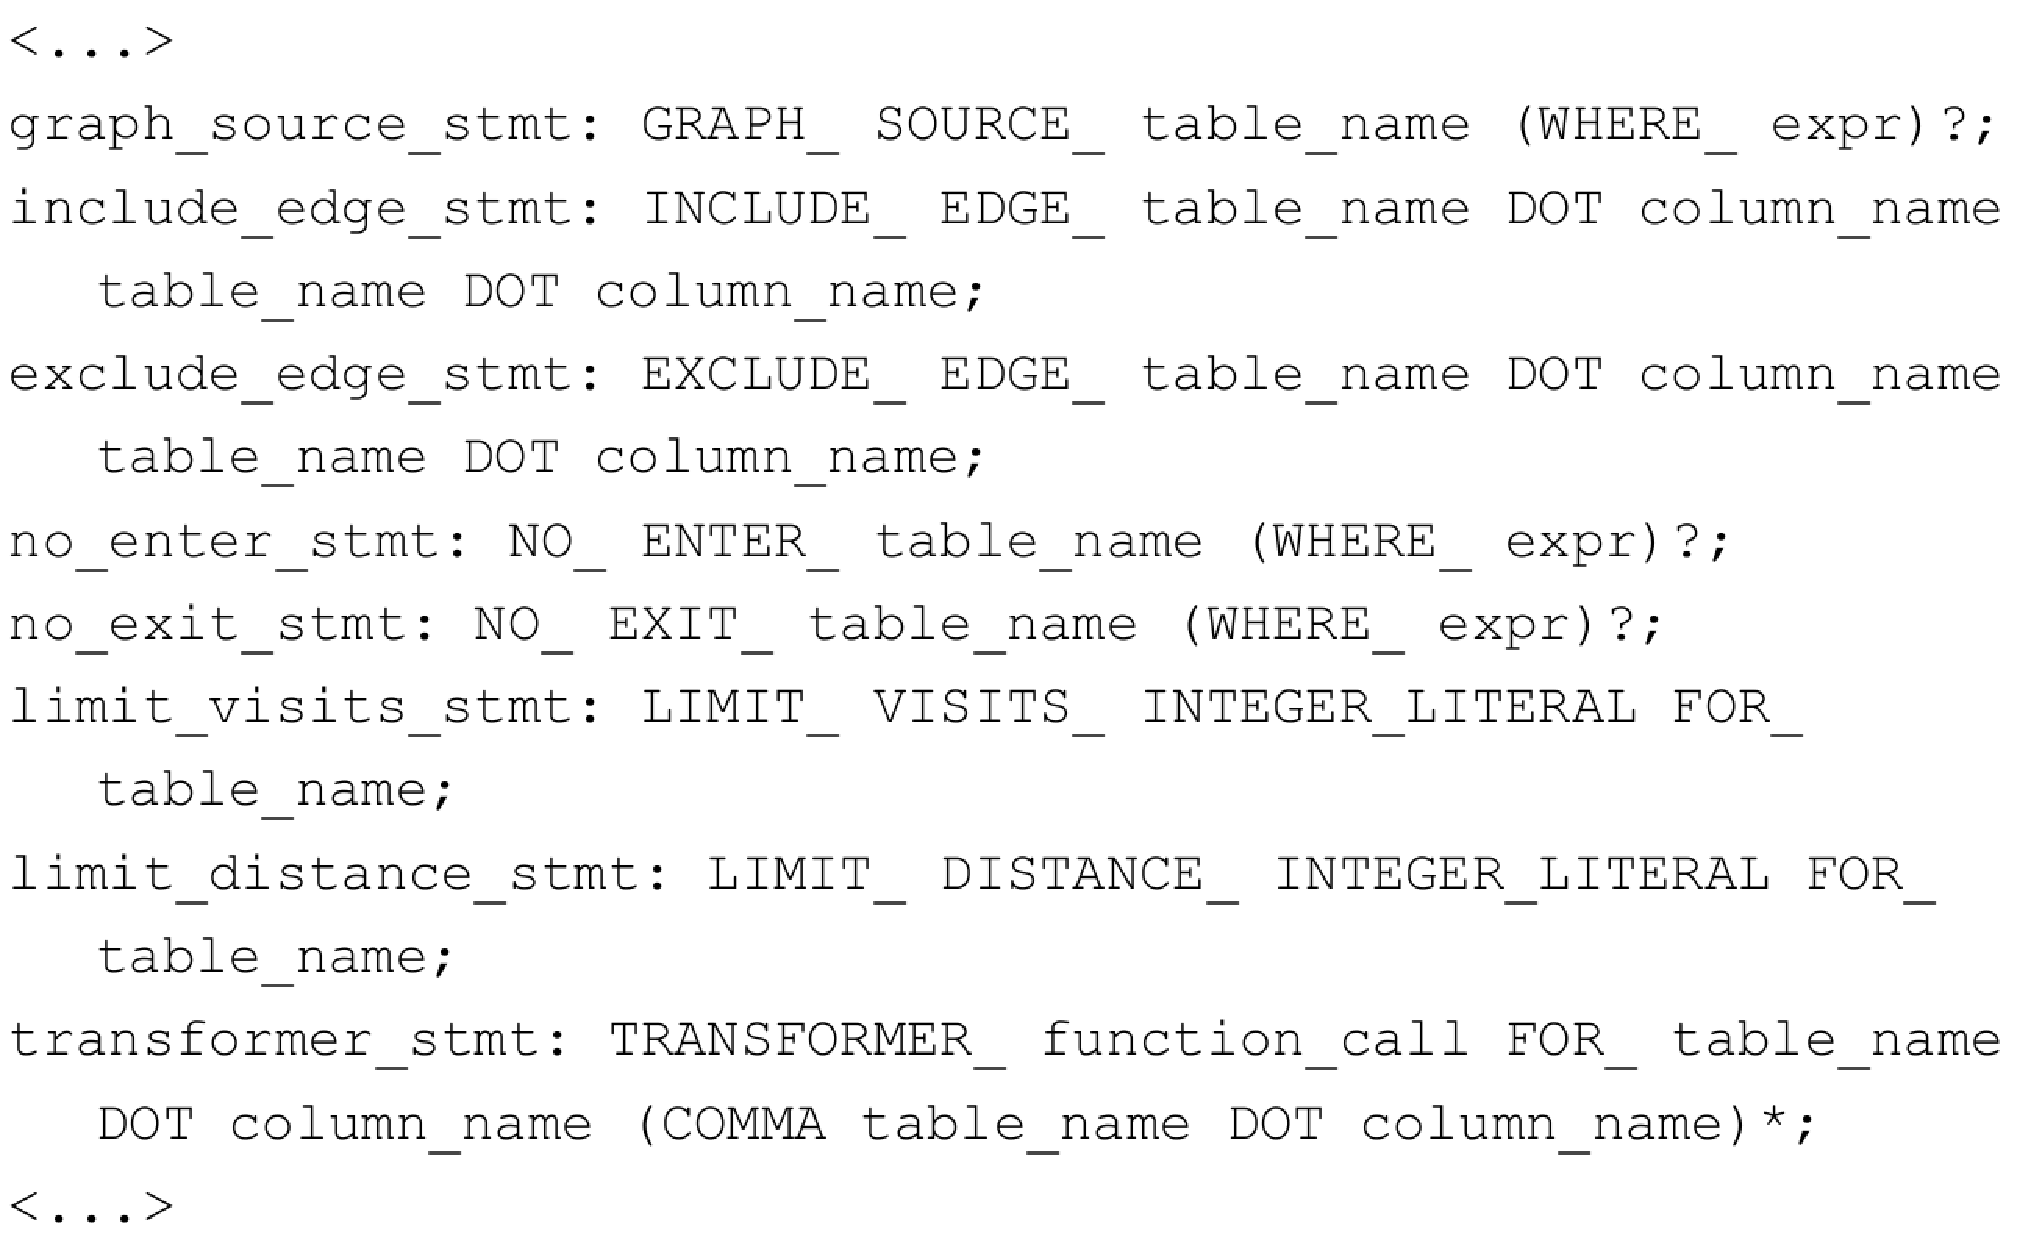
\includegraphics[width = 12cm]{img/grammar}
	\end{center}
\end{frame}


\begin{frame}
\frametitle{Язык описания метаданных}
	Пример описания метаданных для переноса данных

	\begin{center}
		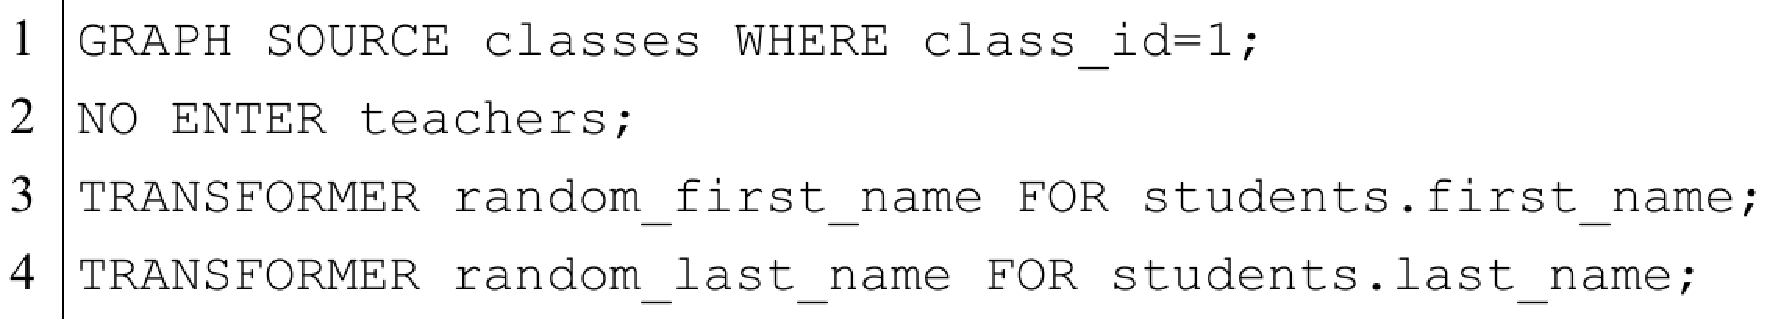
\includegraphics[width = 12cm]{img/language-1}
	\end{center}
\end{frame}


\begin{frame}
\frametitle{Минимально жизнеспособный продукт}
	\textbf{Возможности}:

	\begin{itemize}
		\item интерфейс командной строки;
		\item перенос взаимосвязанных данных;
		\item поддержка правил метаграфа:
		\begin{itemize}
			\item \textit{NO EXIT};
			\item \textit{NO ENTER};
			\item \textit{LIMIT DISTANCE}.
		\end{itemize}
	\end{itemize}
\end{frame}


\begin{frame}
\frametitle{Тесты производительности}
	Тестовая база данных: 4.5 ГБ, 44739072 записей

	\begin{center}
		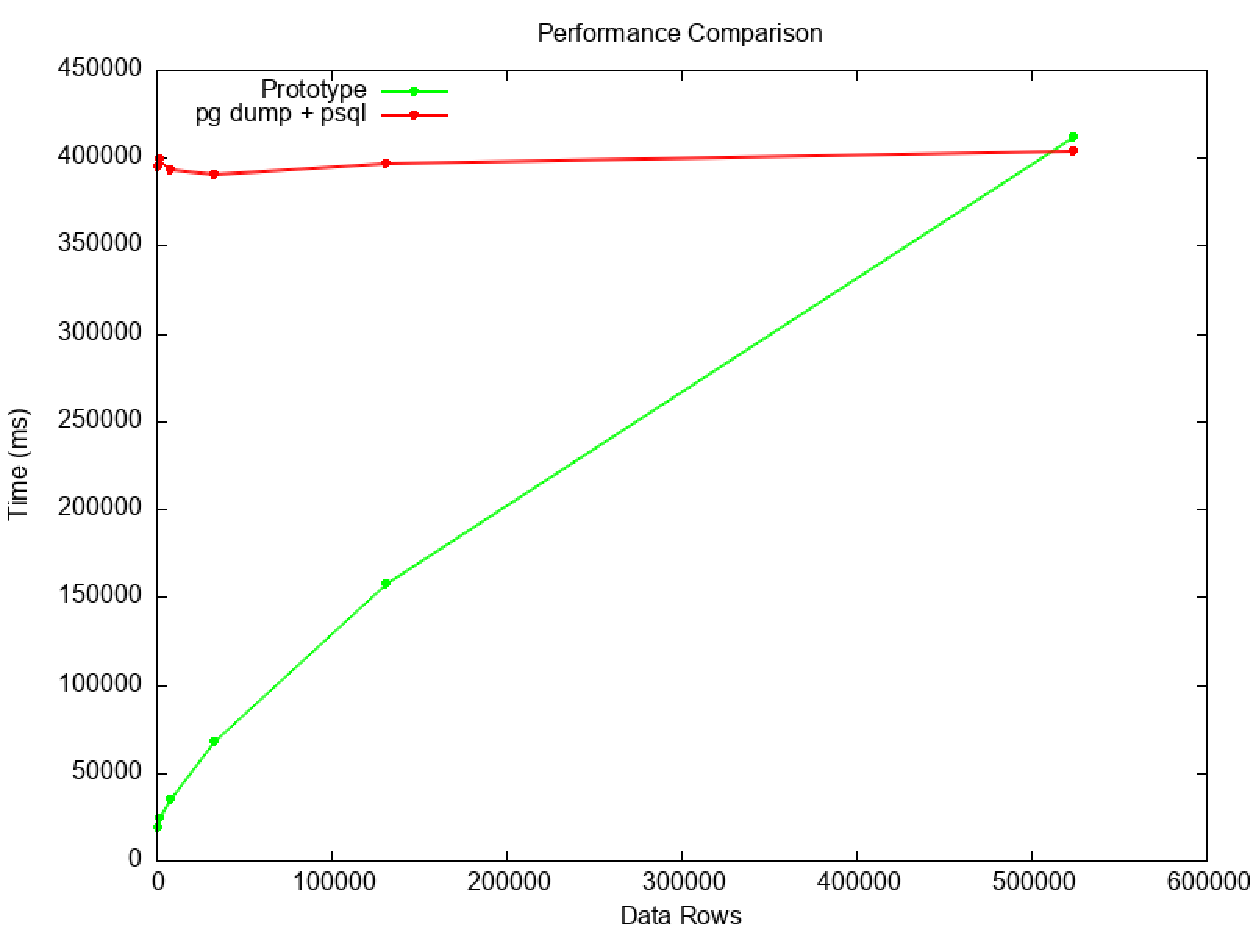
\includegraphics[height = 6cm]{img/benchmark}
	\end{center}
\end{frame}


\begin{frame}
\frametitle{Анализ результатов}
	\textbf{Результаты}:

	\begin{itemize}
		\item спроектирована архитектура, направленная на отказоустойчивость;
		\item разработан язык описания метаданных;
		\item разработан минимально жизнеспособный продукт.
	\end{itemize}

	\textbf{Дальнейшие перспективы}:
	\begin{itemize}
		\item улучшение производительности;
		\item разработка анонимизации и генерации данных.
	\end{itemize}

\end{frame}


\begin{frame}
\frametitle{Описание программной разработки}
	Ссылки на код грамматики и код минимально жизнеспособного продукта

	\begin{center}
		
\includegraphics[height = 6cm]{img/qr-code-relatio-lang}
	\end{center}
\end{frame}

\end{document}
